\chapter{Application windows}

This chapter describes the windows in the program.

\section{Main window}

The main window appears when launching the program and is used as basic interface with the user. It contains the links to get access to the rest of the windows.
\\

\begin{figure}[!h]
\begin{center}
\includegraphics*[height=1.4cm]{images/mprincipalEN.png}
\caption{Initial and main window in the application \emph{surcos}}\label{mainWindow}
\end{center}
\end{figure}

\begin{table}[h]\footnotesize
\begin{center}
\begin{tabular}{llr}
\hline
\multicolumn{2}{c}{Element} \\
\cline{1-2}
Icon & Action & Utility \\
\hline
Exit & Click & Exit the application\\
Open & Click & Open window to load project \\
Configure & Click & Open window to configure project \\
Run & Click & Run project \\
Graphics & Click & Open window for visualization of the results  \\
Summary & Click & Open summary window \\
Help & Click & Information \\
\hline
\end{tabular}
\end{center}
  \caption{Description of the different actions offered by the main menu \emph{surcos}}\label{mainWindowIcons}
\end{table}

Using the icons in table \ref{mainWindowIcons} it is possible to get access to the different utlities in the program.\\
\section{Configuration of a project}
\subsection{Geometry configuration window}

Program \emph{surcos} simulates irrigation in a quadrilateral network of furrows. The geometry configuration window (see figure \ref{geomWindow}) can be used to edit/modify the project topographic data by means of the coordinates of the four vertices that define the furrow plot.

\begin{figure}[!h]
\begin{center}
\includegraphics*[width=\textwidth]{images/confGeomEN.png}
\qquad
\caption{Geometry configuration window}\label{geomWindow}
\end{center}
\end{figure}

As displayed in figure \ref{geomWindow}, the distribution furrow runs between points 1 and 2 and the recirculation furrow, if any, can be defined between points 3 and 4. The irrigation furrows are assumed in the normal direction to the former.

\subsection{Furrow configuration window}

\begin{figure}[!h]
\begin{center}
\includegraphics*[width=\textwidth]{images/confSurcoEN.png}
\qquad
\caption{Furrow configuration window}\label{confSurcos}
\end{center}
\end{figure}

The window displayed in \ref{confSurcos} allows to define the geometric properties of the furrows as divided in three types: distribution, recirculation and irrigation furrows. The different options appear as active or inactive depending on the previous definition of the furrow in our project. The available characteristic to edit are all displayed in figure \ref{confSurcos}.

\subsection{Inlet configuration window}

\begin{figure}[!h]
\begin{center}
\includegraphics*[width=\textwidth]{images/confInputEN.png}
\qquad
\caption{Inlet configuration window}\label{input}
\end{center}
\end{figure}

Window \ref{input} can be used to configure the total water and fertilizer inlet to the furrow system. Every inlet is assigned to a point in the plot where the flow is applied, and is characterized by the initial and the final application times of a constant discharge. The discharge is volumetric rate flow for the water and a mass flow rate for the fertilizer. It is possible to define more complex inlet hydrographs by means of a sequence of inlet discharges at the same point. 

\subsection{Fertilizer configuration window}

\begin{figure}[!h]
\begin{center}
\includegraphics*[width=\textwidth]{images/confFertiEN.png}
\qquad
\caption{Fertilizer configuration window}\label{ferti}
\end{center}
\end{figure}

Window \ref{ferti} is used to state the solubility characteristics of the fertilizer. 

\subsection{Probe configuration window}

\begin{figure}[!h]
\begin{center}
\includegraphics*[width=\textwidth]{images/confSondasEN.png}
\qquad
\caption{Probe configuration window}\label{sondas}
\end{center}
\end{figure}

Window \ref{sondas} can be used to define the number of probes and their location in the plot. Note that, if the point assigned falls out of a furrow, the program finds the nearest position within a furrow.

\subsection{Advanced parameters configuration window}

\begin{figure}[!h]
\begin{center}
\includegraphics*[width=\textwidth]{images/confParam.png}
\qquad
\caption{Advanced parameter configuration window}\label{param}
\end{center}
\end{figure}

Window \ref{param} contains different options to configure the numerical simulation, as follow:

\begin{description}
\item{Maximum simulation time}: Usually, program \emph{surcos} runs the simulation from the initial conditions up to the moment all the applied water has infiltrated in the terrain. In order to avoid excessively long simulation times, this parameter can be used to state a horizon or target time. From that limit, the computation stops even though some water still remains on the surface.
\item{CFL}: Dimensionless numerical parameter proportional to the time step used by the resolution method. It takes values between 0 and 1 for numerical stability reasons. Values close to 1 are optimal. Excessively low values can slow the computation.
\item{Data saving period}: Simulation time interval used to save series of numerical results in a file. It is possible to have $ n=\frac{t_s}{p_v}$ snapshots of the irrigation event, with $ t_s $ the simulation time and $ p_v $ the data saving period.  
\item{Number of cells in the distribution furrow (between irrigation furrows)}: Number of computational cells in the distribution/recirculation furrow between 2 irrigation furrows. (Minimum 3).
\item{Number of cells in the irrigation furrows}: Number of computational cells in every irrigation furrow. More cells implies better quality in the results and slower computations.
\end{description}


\section{Simulation}

After the configuration, the simulation of the project is performed by pressing run in the main menu:

\includegraphics[height=0.4cm]{images/gtk-execute.png}

\section{Results visualization}

%El programa puede mostrar tres tipos de resultados. El primero de ellos es modo textual y los otros dos son en modo gráfico

\subsection{Graphical results}

The graphics are controlled from the window \ref{barraRepres}, where an interactive dial can be used to move forward and backward in time the evolution of the variables represented. It is also possible to choose the furrow, the variable and the probe to view. 

The program offers the possibility to save the graphical results by pressin the button at the bottom of the menu. The image of the plot appearing on the screen in that moment is saved in format \emph{png}.

\begin{figure}[!h]
\begin{center}
\includegraphics*[width=\textwidth]{images/menuRepresEN.png}
\qquad
\caption{Plot selection window}\label{barraRepres}
\end{center}
\end{figure}

Program \emph{Surcos} produces three types of plots. The first is a plan view of the furrow network, with the possibility to display the distribution in the network of the variables described in table \ref{tableVariablesMapa}.

\begin{table}[h]\footnotesize
\begin{center}
\begin{tabular}{ll}
\hline
Variable & Units \\
\hline
Water depth & $m$ \\
Fertilizer concentration & $ kg/m^3 $\\
Infiltrated water volume per unit furrow length & $ m^2 $ \\
Fertilizer mass per unit furrow length & $ kg/m $ \\
\hline
\end{tabular}
\end{center}
  \caption{Variables to view on the furrow network plot}\label{tableVariablesMapa}
\end{table}

\begin{figure}[!h]
\begin{center}
\includegraphics*[width=\textwidth]{images/evo1EN.png}
\qquad
\caption{Example of graphical view in a map of the water depth}\label{evo1}
\end{center}
\end{figure}

The second graphical option is a cartesian XY plot of the longitudinal profile along different furrows. 

The variables that can be plotted in the longitudinal profile are those in table \ref{tableVariables2}.

\begin{table}[h]\footnotesize
\begin{center}
\begin{tabular}{ll}
\hline
Variable & Units\\
\hline
Water depth & $m$ \\
Discharge & $ m^3/s $\\
Surface level (Water surface and bottom) & $ m $\\
Fertilizer concentration & $ kg/m^3 $\\
Surface and infiltrated water volume and fertilizer mass & $ m^2,\;kg/m $ \\
Irrigation advance and recession times & $ s $ \\
\hline
\end{tabular}
\end{center}
  \caption{Variables that can be plotted in every furrow}\label{tableVariables2}
\end{table}

\begin{figure}[!h]
\begin{center}
\includegraphics*[width=\textwidth]{images/evoSurcoEN.png}
\qquad
\caption{Example of the longitudinal profile of the surface and infiltrated water volume and fertilizer mass in a furrow}\label{evo2}
\end{center}
\end{figure}

The third graphical option is a time evolution of the variables in the different probes. These are contained in table \ref{tableVariables3}.

\begin{table}[h]\footnotesize
\begin{center}
\begin{tabular}{llr}
\hline
Variable & Units & Observations \\
\hline
Water depth & $m$ \\
Fertilizer concentration & $ kg/m^3 $\\
\hline
\end{tabular}
\end{center}
  \caption{Variables that can be plotted in a probe.}\label{tableVariables3}
\end{table}

\begin{figure}[!h]
\begin{center}
\includegraphics*[width=\textwidth]{images/evoSondaEN.png}
\qquad
\caption{Example of time evolution at a probe.}\label{evo3}
\end{center}
\end{figure}

\subsection{Summary}

The access to the summary is through the button 
\includegraphics[height=0.4cm]{images/gtk-edit.png}. This is useful to produce a brief text report with the description of the irrigation configuration and the most relevant results obtained. An example is displayed in figure \ref{wInforme}.

The results include the surface, infiltrated and percolated water and fertilizer mass both in the irrigation furrows and in the distribution/recirculation furrows. The infiltrated water mass in the soil that remains available to the crops by retention forces, contrary to the percolated water.

The uniformity of distribution is calculated only in the irrigation furrows. It follows the ratio between the infiltration average of the 25\% of the less irrigated points and the total infiltration average.

Finally, the efficiency is computed as the infiltrated mass in the irrigation furrows divided by the total applied mass. Therefore, both the percolated mass and that present in the distribution/recirculation furrow are considered losses in the estimation of the efficiency. 

The summary window cannot be saved in a file. In order to save the summary data, one option is to select the text with the mouse, copy with the key \emph{Control+C} and paste it in any text editor such as Microsoft Word.


\begin{figure}[!h]
\begin{center}
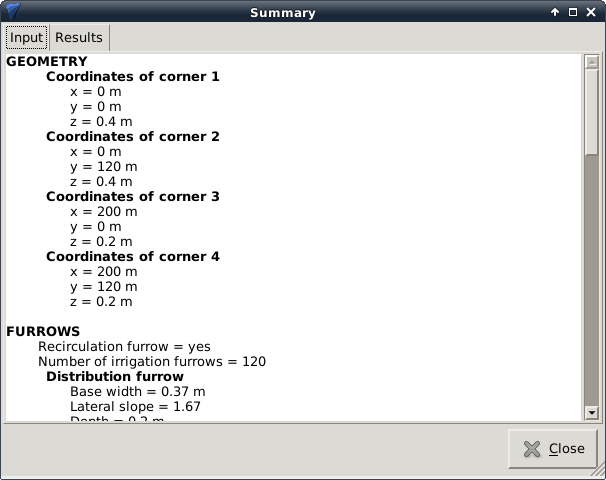
\includegraphics[width=0.45\textwidth]{images/sumarioEN.png}
\qquad
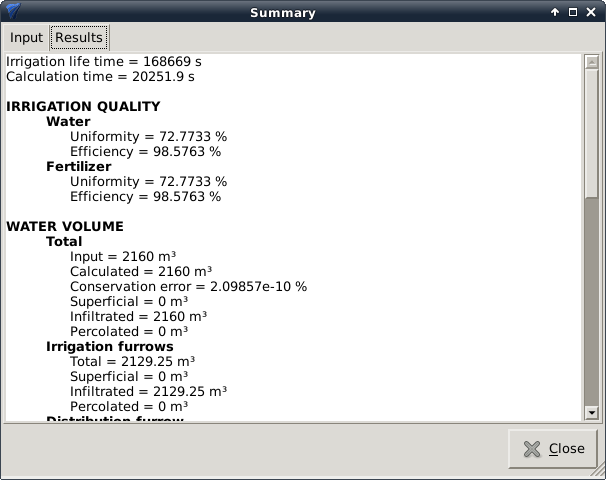
\includegraphics[width=0.45\textwidth]{images/sumario2EN.png}
\caption{Summary of the input data (Left) and results (Right)}\label{wInforme}
\end{center}
\end{figure}


%%%%%%%%%%%%%%%%%%%%%%%%%%%%%%%%%%%%%%%%%%%%%%%%%%%%%%%%%%%%%%%%%%%%%%%%%%%%%%%%%%%%%%%%%%%%%%%%%%%%%%%%5
